\chapter{बहुलक: संश्लेषण, संरचना और गुणधर्म}\label{ch:b2:polymer-synthesis}

नायलॉन के मोज़े 1939 में बिक्री के लिए आए। वे एक ऐसी प्रयोगशाला से निकले थे जिसने कुछ वर्ष
पहले यह समझने का बीड़ा उठाया था कि छोटे अणु लंबे अणुओं में कैसे जुड़ते हैं, और जिसने रास्ते में एक ऐसा
पाठ सीखा था जो हर रसायनज्ञ को पहली बार आश्चर्यचकित करता है: अणुओं को सिरे-से-सिरा जोड़कर बने \omterm{def:b2:polymer-synthesis:polymer}{बहुलक} के लिए
99~\% लब्धि पर्याप्त नहीं है। यह अध्याय बताता है कि क्यों, शृंखलाओं के बढ़ने के दो तरीकों का वर्णन करता है,
और शृंखलाओं की संरचना को पदार्थों के गुणधर्मों से जोड़ता है।
% ledger: hist:nylon-production-1939

\begin{recall}
विद्यालय का खंड: \omterm{def:b2:polymer-synthesis:polymer}{बहुलक}, \omterm{def:b2:polymer-synthesis:polymer}{एकलक} और पुनरावृत्त इकाइयाँ, योगज और संघनन \omterm{def:b2:polymer-synthesis:polymer}{बहुलक},
थर्मोप्लास्टिक और थर्मोसेट। प्रथम वर्ष का खंड: मूलक और समांश विदलन, कार्बधनायन और
कार्बऋणायन, स्थायी-अवस्था सन्निकटन। \Cref{ch:b2:acyl-substitution}: एस्टर और ऐमाइड।
\Cref{ch:b2:catalytic-cycles}: धातु--कार्बन आबंध में निवेशन।
\end{recall}

\section{शृंखलाएँ और उनके मोलर द्रव्यमान}

\begin{definition}[बहुलक]\label{def:b2:polymer-synthesis:polymer}
\emph{बहुलक}\index{बहुलक} वृहदणुओं से बना पदार्थ है, जिनमें से हर एक छोटे अणुओं,
\emph{एकलकों}\index{एकलक}, के बार-बार जुड़ने से बनता है। \emph{पुनरावृत्त इकाई}\index{पुनरावृत्त इकाई}
परमाणुओं का वह सबसे छोटा समूह है जिसकी पुनरावृत्ति से शृंखला बनती है; किसी शृंखला की \emph{बहुलकीकरण की
कोटि}\index{बहुलकीकरण की कोटि} $X$ उसमें उपस्थित एकलक-व्युत्पन्न इकाइयों की संख्या है।
\end{definition}

किसी संश्लेषित \omterm{def:b2:polymer-synthesis:polymer}{बहुलक} का नमूना कभी समान शृंखलाओं से नहीं बना होता: वह
भिन्न लंबाइयों की शृंखलाओं का मिश्रण है, और उसका मोलर द्रव्यमान एक औसत है, जो इस पर निर्भर करता है कि शृंखलाएँ कैसे गिनी जाती हैं।

\begin{definition}[मोलर-द्रव्यमान औसत]\label{def:b2:polymer-synthesis:averages}
किसी नमूने के लिए जिसमें $N_i$ शृंखलाएँ हों, मोलर द्रव्यमान $M_i$ की, \emph{संख्या-औसत मोलर
द्रव्यमान}\index{संख्या-औसत मोलर द्रव्यमान} और \emph{द्रव्यमान-औसत मोलर द्रव्यमान}\index{द्रव्यमान-औसत मोलर द्रव्यमान}
ये हैं:
\begin{equation*}
\bar M_n = \frac{\sum_i N_i M_i}{\sum_i N_i}, \qquad
\bar M_w = \frac{\sum_i N_i M_i^2}{\sum_i N_i M_i} = \sum_i w_i M_i,
\end{equation*}
जहाँ $w_i$ द्रव्यमान $M_i$ वाली शृंखलाओं का द्रव्यमान अंश है। \emph{परिक्षेपिता}\index{परिक्षेपिता}
$\text{\DH} = \bar M_w/\bar M_n$ कम-से-कम 1 है, और 1 के बराबर तभी जब सभी शृंखलाओं का द्रव्यमान
समान हो। \omterm{def:b2:polymer-synthesis:polymer}{बहुलकीकरण की कोटि} के औसत $\bar X_n$ और $\bar X_w$ इसी प्रकार परिभाषित
होते हैं।
\end{definition}

संख्या-औसत हर शृंखला को एक बार भारित करता है; द्रव्यमान-औसत हर शृंखला को उसके द्रव्यमान से भारित करता है, अतः
लंबी शृंखलाएँ अधिक गिनी जाती हैं। $\text{\DH} \ge 1$ असमिका $\left(\sum N_i M_i\right)^2 \le
\sum N_i \sum N_i M_i^2$ (कोशी--श्वार्ज़) है, जिसमें समता केवल समान $M_i$ के लिए होती है।

\begin{method}[औसतों का परिकलन]\label{met:b2:polymer-synthesis:averages}
\begin{enumerate}
  \item आँकड़ों को मात्राओं $N_i$ (या शृंखलाओं की संख्याओं) और द्रव्यमानों $M_i$ में बदलिए; द्रव्यमान अंशों से
        $N_i \propto w_i/M_i$।
  \item $\bar M_n = \sum N_i M_i / \sum N_i$; तुल्य रूप से, $1/\bar M_n = \sum w_i/M_i$।
  \item $\bar M_w = \sum w_i M_i$।
  \item $\text{\DH} = \bar M_w/\bar M_n$; जाँचिए कि $\bar M_w \ge \bar M_n$।
\end{enumerate}
\end{method}

\section{चरण-वृद्धि और शृंखला-वृद्धि}

\begin{definition}[चरण-वृद्धि और शृंखला-वृद्धि]\label{def:b2:polymer-synthesis:step-chain}
\emph{चरण-वृद्धि बहुलकीकरण}\index{चरण-वृद्धि बहुलकीकरण} में पूरक क्रियात्मक समूह धारण करने वाले कोई भी दो अणु
(\omterm{def:b2:polymer-synthesis:polymer}{एकलक}, अल्पलक या लंबी शृंखलाएँ) अभिक्रिया कर सकते हैं, और शृंखलाएँ
एक-दूसरे से जुड़कर लंबी होती हैं: पॉलिएस्टर, पॉलिऐमाइड। \emph{शृंखला-वृद्धि
बहुलकीकरण}\index{शृंखला-वृद्धि बहुलकीकरण} में कोई अभिक्रियाशील केंद्र (मूलक, आयन या धातु--कार्बन
आबंध) बढ़ती शृंखला के सिरे पर एक-एक करके \omterm{def:b2:polymer-synthesis:polymer}{एकलक} अणु जोड़ता है: ऐल्कीनों के \omterm{def:b2:polymer-synthesis:polymer}{बहुलक}।
\end{definition}

\begin{method}[चरण या शृंखला?]\label{met:b2:polymer-synthesis:classify}
\begin{enumerate}
  \item दो क्रियात्मक समूहों वाला \omterm{def:b2:polymer-synthesis:polymer}{एकलक} जो एक-दूसरे के भागीदार से अभिक्रिया करते हैं (अम्ल और ऐल्कोहॉल,
        अम्ल और ऐमीन), प्रायः कोई छोटा अणु मुक्त करते हुए: चरण-वृद्धि।
  \item \ce{C=C} द्वि-आबंध (या तनावग्रस्त वलय) वाला \omterm{def:b2:polymer-synthesis:polymer}{एकलक} और एक आरंभक: शृंखला-वृद्धि।
  \item अभिक्रिया की प्रगति से जाँचिए: चरण-वृद्धि में \omterm{def:b2:polymer-synthesis:polymer}{एकलक} जल्दी समाप्त हो जाता है और लंबी शृंखलाएँ
        केवल बिल्कुल अंत में दिखती हैं; शृंखला-वृद्धि में लंबी शृंखलाएँ आरंभ से ही दिखती हैं जबकि \omterm{def:b2:polymer-synthesis:polymer}{एकलक}
        धीरे-धीरे उपभुक्त होता है।
\end{enumerate}
\end{method}

\subsection*{चरण-वृद्धि}

\ce{A-A} और \ce{B-B} \omterm{def:b2:polymer-synthesis:polymer}{एकलकों} (एक डाइऐमीन और एक डाइअम्ल) का एक संतुलित मिश्रण लीजिए, या एक अकेला
\ce{A-B} \omterm{def:b2:polymer-synthesis:polymer}{एकलक}। $p$ को \emph{अभिक्रिया की प्रगति} कहिए: एक प्रकार के क्रियात्मक समूहों का
वह अंश जिसने अभिक्रिया कर ली है।

\begin{theorem}[कैरोदर्स समीकरण]\label{thm:b2:polymer-synthesis:carothers}
ठीक-ठीक संतुलित द्विक्रियाशील \omterm{def:b2:polymer-synthesis:polymer}{एकलकों} के \omterm{def:b2:polymer-synthesis:step-chain}{चरण-वृद्धि बहुलकीकरण} में, \omterm{def:b2:polymer-synthesis:polymer}{एकलक} इकाइयों में गिनी गई,
संख्या-औसत \omterm{def:b2:polymer-synthesis:polymer}{बहुलकीकरण की कोटि} यह है:
\begin{equation*}
\bar X_n = \frac{1}{1 - p}.
\end{equation*}
\end{theorem}

\begin{proof}
$N_0$ \omterm{def:b2:polymer-synthesis:polymer}{एकलक} अणुओं से आरंभ कीजिए, जो $N_0$ समूह \ce{A} और $N_0$ समूह \ce{B} धारण करते हैं। किसी \ce{A} और
किसी \ce{B} के बीच हर अभिक्रिया दो अणुओं को एक में जोड़ती है, अतः अणुओं की संख्या को
एक घटाती है। $pN_0$ अभिक्रियाओं के बाद $N = N_0 - pN_0 = N_0(1-p)$ अणु बचते हैं जो $N_0$ \omterm{def:b2:polymer-synthesis:polymer}{एकलक}
इकाइयों को साझा करते हैं: $\bar X_n = N_0/N = 1/(1-p)$।
\end{proof}

\begin{corollary}[असंतुलन]\label{cor:b2:polymer-synthesis:imbalance}
यदि समूह संतुलित नहीं हैं, $r = N_{\ce{A}}/N_{\ce{B}} \le 1$ के साथ और $p$ को अल्पसंख्यक समूहों \ce{A}
की अभिक्रिया की प्रगति मानकर,
\begin{equation*}
\bar X_n = \frac{1 + r}{1 + r - 2rp}, \qquad \text{अधिकतम } \frac{1+r}{1-r} \text{, जब } p = 1.
\end{equation*}
\end{corollary}

\begin{proof}
प्रारंभ में $(N_{\ce{A}} + N_{\ce{B}})/2$ द्विक्रियाशील \omterm{def:b2:polymer-synthesis:polymer}{एकलक} अणु हैं। हर रैखिक
अणु के दो शृंखला-सिरे होते हैं, हर एक एक अनभिक्रियित समूह; अभिक्रिया के बाद $N_{\ce{A}}(1-p)$
समूह \ce{A} और $N_{\ce{B}} - pN_{\ce{A}}$ समूह \ce{B} बचते हैं, अतः $N = [N_{\ce{A}}(1-p) + N_{\ce{B}} -
pN_{\ce{A}}]/2$ अणु। भाग देने पर, $N_{\ce{B}} = N_{\ce{A}}/r$ के साथ:
$\bar X_n = (1 + 1/r)/(1 - 2p + 1/r) = (1+r)/(1 + r - 2rp)$। $r = 1$ के साथ यही कैरोदर्स समीकरण है।
\end{proof}

यह समीकरण आरंभ की पहेली को समझाता है। $p = 0.99$ पर, अर्थात् जोड़ने वाली अभिक्रिया की ``99~\% लब्धि'' पर, $\bar X_n =
100$; किसी उपयोगी रेशे को लगभग इतनी या अधिक चाहिए, अतः जोड़ने की प्रक्रिया 99~\% से आगे जानी चाहिए, शुद्ध \omterm{def:b2:polymer-synthesis:polymer}{एकलकों}
के साथ ठीक-ठीक समान मात्राओं में, और मुक्त होने वाले छोटे अणु (जल, मेथेनॉल) को हटाते हुए ताकि
साम्य आगे धकेला जाता रहे। किसी एक \omterm{def:b2:polymer-synthesis:polymer}{एकलक} का 1~\% आधिक्य पूर्ण \omterm{def:b2:continuous-reactors:conversion}{रूपांतरण} पर भी $\bar X_n$ को 201 पर सीमित कर देता है।

\begin{theorem}[फ़्लोरी वितरण]\label{thm:b2:polymer-synthesis:flory}
प्रगति $p$ पर किसी \omterm{def:b2:polymer-synthesis:step-chain}{चरण-वृद्धि बहुलकीकरण} में, यदि हर समूह की अभिक्रियाशीलता उसकी शृंखला की लंबाई चाहे जो हो
समान रहे, तो $x$ इकाइयों वाली शृंखलाओं का संख्या अंश और द्रव्यमान अंश ये हैं:
\begin{equation*}
n_x = (1-p)\,p^{\,x-1}, \qquad w_x = x(1-p)^2 p^{\,x-1},
\end{equation*}
और $\bar X_n = 1/(1-p)$, $\bar X_w = (1+p)/(1-p)$, जिससे $\text{\DH} = 1 + p$, जो उच्च
\omterm{def:b2:continuous-reactors:conversion}{रूपांतरण} पर 2 के निकट है।
\end{theorem}

\begin{proof}
किसी शृंखला का एक सिरे से अनुसरण कीजिए (सरलता के लिए एक \ce{A-B} \omterm{def:b2:polymer-synthesis:polymer}{एकलक})। उसके अनुदिश हर कड़ी
प्रायिकता $p$ से, स्वतंत्र रूप से, बनती है। शृंखला में ठीक $x$ इकाइयाँ होती हैं यदि पहली $x-1$ कड़ियाँ बनें
और अगली न बने: प्रायिकता $p^{\,x-1}(1-p)$, जो $n_x$ है। $\sum_{x\ge1} p^{\,x-1} =
1/(1-p)$ और उसके अवकलजों $\sum x p^{\,x-1} = 1/(1-p)^2$ और $\sum x^2 p^{\,x-1} = (1+p)/(1-p)^3$ के साथ:
$\sum n_x = 1$, $\bar X_n = \sum x n_x = 1/(1-p)$, $w_x = x n_x/\bar X_n = x(1-p)^2p^{\,x-1}$, और
$\bar X_w = \sum x w_x = (1-p)^2(1+p)/(1-p)^3 = (1+p)/(1-p)$।
\end{proof}

\begin{omfigure}
\begin{tikzpicture}
\begin{axis}[width=0.46\linewidth, height=5cm, xmin=0, xmax=400, ymin=0,
  xlabel={बहुलकीकरण की कोटि $x$}, ylabel={द्रव्यमान अंश $w_x$}, label style={font=\small},
  tick label style={font=\scriptsize}, scaled y ticks=false,
  yticklabel style={/pgf/number format/fixed, /pgf/number format/precision=3},
  legend style={font=\scriptsize, at={(0.98,0.98)}, anchor=north east}, legend cell align=left]
\addplot[omDef, thick] table[x=x, y=p95] {figdata/out/bachelor-2-polymer-distributions-a.dat};
\addplot[omThm, thick] table[x=x, y=p98] {figdata/out/bachelor-2-polymer-distributions-a.dat};
\addplot[omMeth, thick] table[x=x, y=p99] {figdata/out/bachelor-2-polymer-distributions-a.dat};
\legend{$p = 0.95$, $p = 0.98$, $p = 0.99$}
\end{axis}
\end{tikzpicture}\hfill
\begin{tikzpicture}
\begin{axis}[width=0.46\linewidth, height=5cm, xmin=0, xmax=1, ymin=0, ymax=200,
  xlabel={अभिक्रिया की प्रगति $p$}, ylabel={$\bar X_n$}, label style={font=\small},
  tick label style={font=\scriptsize}, xtick={0,0.2,0.4,0.6,0.8,1}]
\addplot[omDef, thick] table[x=p, y=Xn] {figdata/out/bachelor-2-polymer-distributions-b.dat};
\end{axis}
\end{tikzpicture}

{\small \omterm{def:b2:polymer-synthesis:step-chain}{चरण-वृद्धि बहुलकीकरण} (मॉडल)। बाएँ: फ़्लोरी द्रव्यमान वितरण
(\cref{thm:b2:polymer-synthesis:flory}); शिखर $\bar X_n$ के निकट है और वितरण
बाहर खिसकने के साथ चौड़ा होता है। दाएँ: कैरोदर्स समीकरण; $\bar X_n$ तब तक छोटा रहता है जब तक $p$ 1 के अत्यंत निकट न हो।}
% figdata: bachelor-2/polymer-distributions.py parts a, b
\end{omfigure}

\subsection*{मूलक शृंखला-वृद्धि}

\begin{definition}[शृंखला बहुलकीकरण के चरण]\label{def:b2:polymer-synthesis:chain-steps}
मूलक शृंखला बहुलकीकरण तीन प्रकार के चरणों में चलता है। \emph{आरंभन}\index{आरंभन} में कोई
\emph{मूलक आरंभक}\index{मूलक आरंभक} (दुर्बल आबंध वाला अणु, जैसे कोई परॉक्साइड या कोई
ऐज़ो यौगिक) गर्म करने पर मूलकों में टूटता है, जिनमें से एक किसी \omterm{def:b2:polymer-synthesis:polymer}{एकलक} से जुड़ता है। \emph{संचरण}\index{संचरण}
में शृंखला-सिरे का मूलक एक \omterm{def:b2:polymer-synthesis:polymer}{एकलक} अणु जोड़ता है और मूलक ही बना रहता है। \emph{समापन}\index{समापन} में
दो मूलक एक-दूसरे को नष्ट करते हैं, संयोजन द्वारा (वे आबंधित होते हैं) या असमानुपातन द्वारा (एक दूसरे से एक
हाइड्रोजन परमाणु ले लेता है)।
\end{definition}

\begin{omfigure}
\begin{align*}
&\text{आरंभन:} && \mathrm{I{-}I} \longrightarrow 2\,\mathrm{I^{\bullet}}, \qquad
\mathrm{I^{\bullet} + CH_2{=}CHPh \longrightarrow I{-}CH_2{-}\dot{C}HPh} \\
&\text{संचरण:} && {\sim}\mathrm{CH_2{-}\dot{C}HPh + CH_2{=}CHPh \longrightarrow}\;
{\sim}\mathrm{CH_2{-}CHPh{-}CH_2{-}\dot{C}HPh} \\
&\text{समापन:} && {\sim}\mathrm{CH_2{-}\dot{C}HPh + Ph\dot{C}H{-}CH_2}{\sim} \longrightarrow
{\sim}\mathrm{CH_2{-}CHPh{-}CHPh{-}CH_2}{\sim}
\end{align*}

{\small स्टाइरीन का मूलक बहुलकीकरण। आरंभक \ce{I-I} (उदाहरण के लिए डाइबेन्ज़ॉयल परॉक्साइड)
दो मूलकों में टूटता है; हर एक स्टाइरीन के \ce{CH2} सिरे से जुड़ता है, जिससे अधिक स्थायी बेन्ज़िलिक
मूलक मिलता है; \omterm{def:b2:polymer-synthesis:chain-steps}{संचरण} योग को हज़ारों बार दोहराता है; दो शृंखला मूलक संयोजित होकर दोनों
शृंखलाओं को समाप्त कर देते हैं। बिंदु अयुग्मित इलेक्ट्रॉन को दर्शाता है।}
\end{omfigure}

\begin{theorem}[मूलक बहुलकीकरण की दर]\label{thm:b2:polymer-synthesis:radical-rate}
दर स्थिरांक $k_d$ और दक्षता $f$ (शृंखला आरंभ करने वाले मूलकों का अंश) से विघटित होने वाले आरंभक,
\omterm{def:b2:polymer-synthesis:chain-steps}{संचरण} स्थिरांक $k_p$ और \omterm{def:b2:polymer-synthesis:chain-steps}{समापन} स्थिरांक $k_t$ (\omterm{def:b2:polymer-synthesis:chain-steps}{समापन} दर $2k_t
[\mathrm{M^\bullet}]^2$) के साथ बहुलकीकरण की स्थायी-अवस्था दर यह है:
\begin{equation*}
R_p = k_p [\mathrm M] \sqrt{\frac{f k_d [\mathrm I]}{k_t}}.
\end{equation*}
\end{theorem}

\begin{proof}
$[\mathrm{M^\bullet}]$ को शृंखला मूलकों की कुल सांद्रता मानिए, उनकी लंबाई चाहे जो हो। वे
दर $R_i = 2fk_d[\mathrm I]$ से बनते हैं (प्रति आरंभक अणु दो मूलक, जिनमें से अंश $f$
शृंखलाएँ आरंभ करता है) और दर $2k_t[\mathrm{M^\bullet}]^2$ से नष्ट होते हैं; \omterm{def:b2:polymer-synthesis:chain-steps}{संचरण} एक शृंखला
मूलक को दूसरे में बदलता है और उनकी संख्या नहीं बदलता। $[\mathrm{M^\bullet}]$ पर स्थायी-अवस्था सन्निकटन
$2fk_d[\mathrm I] = 2k_t[\mathrm{M^\bullet}]^2$ देता है, अतः $[\mathrm{M^\bullet}] =
\sqrt{fk_d[\mathrm I]/k_t}$। \omterm{def:b2:polymer-synthesis:polymer}{एकलक} का उपभोग अनिवार्यतः \omterm{def:b2:polymer-synthesis:chain-steps}{संचरण} द्वारा होता है, दर $R_p =
k_p[\mathrm M][\mathrm{M^\bullet}]$ पर।
\end{proof}

\begin{definition}[गतिक शृंखला लंबाई]\label{def:b2:polymer-synthesis:chain-length}
\emph{गतिक शृंखला लंबाई}\index{गतिक शृंखला लंबाई} $\nu$ शृंखला आरंभ करने वाले प्रति मूलक जोड़े गए \omterm{def:b2:polymer-synthesis:polymer}{एकलक}
अणुओं की औसत संख्या है: $\nu = R_p/R_i$।
\end{definition}

\begin{proposition}[शृंखला लंबाई और आरंभक]\label{prop:b2:polymer-synthesis:chain-length}
स्थायी अवस्था में $\nu = k_p[\mathrm M]/\bigl(2\sqrt{fk_dk_t[\mathrm I]}\bigr)$: अधिक आरंभक
तेज़ बहुलकीकरण परंतु छोटी शृंखलाएँ देता है। संयोजन द्वारा \omterm{def:b2:polymer-synthesis:chain-steps}{समापन} के साथ $\bar X_n = 2\nu$;
असमानुपातन द्वारा, $\bar X_n = \nu$।
\end{proposition}

\begin{proof}
$\nu = R_p/R_i = k_p[\mathrm M]\sqrt{fk_d[\mathrm I]/k_t}/(2fk_d[\mathrm I]) =
k_p[\mathrm M]/\bigl(2\sqrt{fk_dk_t[\mathrm I]}\bigr)$। आरंभ हुई हर शृंखला औसतन $\nu$ \omterm{def:b2:polymer-synthesis:polymer}{एकलक} जोड़ती है;
संयोजन ऐसी दो शृंखलाओं को एक अणु में जोड़ता है, असमानुपातन दो ही छोड़ता है।
\end{proof}

\begin{definition}[सजीव बहुलकीकरण]\label{def:b2:polymer-synthesis:living}
\emph{सजीव बहुलकीकरण}\index{सजीव बहुलकीकरण} बिना \omterm{def:b2:polymer-synthesis:chain-steps}{समापन} या
स्थानांतरण वाला \omterm{def:b2:polymer-synthesis:step-chain}{शृंखला-वृद्धि बहुलकीकरण} है: सभी शृंखलाएँ एक साथ आरंभ होती हैं और जब तक \omterm{def:b2:polymer-synthesis:polymer}{एकलक} बचा है बढ़ती रहती हैं, और
और \omterm{def:b2:polymer-synthesis:polymer}{एकलक} मिलाने पर फिर बढ़ने लगती हैं। किसी शुष्क, अप्रोटिक विलायक में ब्यूटिललिथियम द्वारा आरंभित
स्टाइरीन का ऋणायनी बहुलकीकरण इसका शास्त्रीय उदाहरण है।
\end{definition}

\begin{proposition}[संकीर्ण वितरण]\label{prop:b2:polymer-synthesis:living}
ऐसे \omterm{def:b2:polymer-synthesis:living}{सजीव बहुलकीकरण} में जिसमें सभी शृंखलाएँ एक साथ आरंभ हों, \omterm{def:b2:polymer-synthesis:polymer}{बहुलकीकरण की कोटि}
प्वासों वितरण का अनुसरण करती है, और $\text{\DH} = 1 + \nu/(1+\nu)^2 \approx 1 + 1/\bar X_n$, जहाँ $\nu$
प्रति शृंखला जोड़े गए \omterm{def:b2:polymer-synthesis:polymer}{एकलकों} की माध्य संख्या है।
\end{proposition}

\admitted

यह वितरण योगों की संख्या का है, जो हर शृंखला द्वारा उसी समय में एक उभयनिष्ठ दर पर
किए गए स्वतंत्र यादृच्छिक घटनाएँ हैं; \omterm{def:b2:polymer-synthesis:averages}{परिक्षेपिता} प्वासों नियम के माध्य और प्रसरण से निकलती है,
जो दोनों $\nu$ के बराबर हैं। इस प्रकार 100 इकाइयों की सजीव शृंखला का $\text{\DH} \approx 1.01$ है, जबकि
चरण-वृद्धि द्वारा बने उसी औसत के लिए लगभग 2।
\begin{omfigure}
\begin{tikzpicture}
\begin{axis}[width=0.72\linewidth, height=5cm, xmin=0, xmax=150, ymin=0,
  xlabel={बहुलकीकरण की कोटि $x$}, ylabel={द्रव्यमान अंश $w_x$}, label style={font=\small},
  tick label style={font=\scriptsize}, scaled y ticks=false,
  yticklabel style={/pgf/number format/fixed, /pgf/number format/precision=3},
  legend style={font=\scriptsize, at={(0.98,0.98)}, anchor=north east}, legend cell align=left]
\addplot[omThm, thick] table[x=x, y=poisson] {figdata/out/bachelor-2-polymer-distributions-c.dat};
\addplot[omDef, thick] table[x=x, y=flory] {figdata/out/bachelor-2-polymer-distributions-c.dat};
\legend{सजीव (प्वासों), चरण-वृद्धि (फ़्लोरी)}
\end{axis}
\end{tikzpicture}

{\small समान $\bar X_n = 50$ वाले दो नमूने (मॉडल)। सजीव शृंखलाएँ 50 के आसपास सिमटी रहती हैं ($\text{\DH}
\approx 1.02$); चरण-वृद्धि शृंखलाएँ \omterm{def:b2:polymer-synthesis:polymer}{एकलक} से लेकर कई सौ इकाइयों तक फैली होती हैं ($\text{\DH} \approx
1.98$)।}
% figdata: bachelor-2/polymer-distributions.py part c
\end{omfigure}

\begin{definition}[सहबहुलक]\label{def:b2:polymer-synthesis:copolymer}
\emph{सहबहुलक}\index{सहबहुलक} दो या अधिक भिन्न \omterm{def:b2:polymer-synthesis:polymer}{एकलकों} से बना \omterm{def:b2:polymer-synthesis:polymer}{बहुलक} है। इसकी इकाइयाँ
यादृच्छिक रूप से एक-दूसरे के बाद आ सकती हैं (सांख्यिकीय सहबहुलक), एकांतर रूप से, हर एक की लंबी शृंखलाओं में (ब्लॉक
सहबहुलक, \omterm{def:b2:polymer-synthesis:living}{सजीव बहुलकीकरण} से बना), या एक की पार्श्व शृंखलाओं के रूप में जो दूसरे की मुख्य शृंखला पर रोपित हों
(रोपित सहबहुलक)।
\end{definition}

\section{शृंखलाओं की संरचना}

\begin{definition}[टैक्टिसिटी]\label{def:b2:polymer-synthesis:tacticity}
किसी वाइनिल \omterm{def:b2:polymer-synthesis:polymer}{बहुलक} \ce{-[CH2-CHR]_n-} में हर \ce{CHR} कार्बन एक त्रिविमजनक केंद्र है।
\emph{टैक्टिसिटी}\index{टैक्टिसिटी} समतलीय टेढ़ी-मेढ़ी रेखा के रूप में खींची गई शृंखला के अनुदिश उनके आपेक्षिक
विन्यासों का वर्णन करती है: \emph{आइसोटैक्टिक}\index{आइसोटैक्टिक} शृंखला में सभी \ce{R} समूह तल की
एक ही ओर होते हैं, \emph{सिंडियोटैक्टिक}\index{सिंडियोटैक्टिक} शृंखला में वे एकांतर होते हैं, और
\emph{ऐटैक्टिक}\index{ऐटैक्टिक} शृंखला में यादृच्छिक रूप से स्थित होते हैं।
\end{definition}

\begin{omfigure}
\setchemfig{atom sep=1.5em}
\begin{tabular}{rl}
\small \omterm{def:b2:polymer-synthesis:tacticity}{आइसोटैक्टिक} & \chemfig{[:-30]-[:30](<[:90])-[:-30]-[:30](<[:90])-[:-30]-[:30](<[:90])-[:-30]-[:30](<[:90])-[:-30]-[:30](<[:90])-[:-30]} \\[2pt]
\small \omterm{def:b2:polymer-synthesis:tacticity}{सिंडियोटैक्टिक} & \chemfig{[:-30]-[:30](<[:90])-[:-30]-[:30](<:[:90])-[:-30]-[:30](<[:90])-[:-30]-[:30](<:[:90])-[:-30]-[:30](<[:90])-[:-30]} \\[2pt]
\small \omterm{def:b2:polymer-synthesis:tacticity}{ऐटैक्टिक} & \chemfig{[:-30]-[:30](<[:90])-[:-30]-[:30](<[:90])-[:-30]-[:30](<:[:90])-[:-30]-[:30](<[:90])-[:-30]-[:30](<:[:90])-[:-30]}
\end{tabular}
\par\vspace{6pt}

{\small पृष्ठ के तल में टेढ़ी-मेढ़ी रेखा के रूप में खींचा गया पॉलिप्रोपीन; हर मेथिल समूह एक फान है (पाठक की
ओर) या एक रेखांकित फान (दूर)। \omterm{def:b2:polymer-synthesis:tacticity}{आइसोटैक्टिक}: सभी मेथिल एक ओर; \omterm{def:b2:polymer-synthesis:tacticity}{सिंडियोटैक्टिक}: एकांतर;
\omterm{def:b2:polymer-synthesis:tacticity}{ऐटैक्टिक}: अनियमित।}
\end{omfigure}

नियमित शृंखलाएँ अगल-बगल संकुलित होकर क्रिस्टलीय क्षेत्र बना सकती हैं; अनियमित नहीं। \omterm{def:b2:polymer-synthesis:tacticity}{आइसोटैक्टिक}
पॉलिप्रोपीन, जो तृतीय वर्ष के खंड के धातु उत्प्रेरकों से बनता है, आंशिक रूप से क्रिस्टलीय, कठोर और उच्च
गलनांक वाला है; \omterm{def:b2:polymer-synthesis:tacticity}{ऐटैक्टिक} पॉलिप्रोपीन एक मुलायम, चिपचिपा अक्रिस्टलीय पदार्थ है। कोई \omterm{def:b2:polymer-synthesis:polymer}{बहुलक} शायद ही कभी पूर्णतः
क्रिस्टलीय होता है: क्रिस्टलक अक्रिस्टलीय क्षेत्रों में धँसे होते हैं जहाँ शृंखलाएँ उलझी होती हैं।

\begin{definition}[ऊष्मीय संक्रमण]\label{def:b2:polymer-synthesis:transitions}
किसी \omterm{def:b2:polymer-synthesis:polymer}{बहुलक} की \emph{क्रिस्टलता की कोटि}\index{क्रिस्टलता की कोटि} उसका वह द्रव्यमान अंश है
जो क्रिस्टलीय क्षेत्रों में स्थित है। \emph{काँच संक्रमण ताप}\index{काँच संक्रमण ताप}
$T_g$ वह ताप है जिसके नीचे अक्रिस्टलीय क्षेत्र एक दृढ़ काँच होते हैं, उनके शृंखला
खंड गति करने में असमर्थ, और जिसके ऊपर वे रबर जैसे हो जाते हैं; क्रिस्टलीय क्षेत्र एक उच्चतर
ताप, $T_m$, पर पिघलते हैं।
\end{definition}

पॉलिस्टाइरीन और पॉली(मेथिल मेथैक्रिलेट) अक्रिस्टलीय हैं और उनका $T_g$ कमरे के ताप से ऊपर है: दृढ़,
पारदर्शी काँच। प्राकृतिक रबर का $T_g$ कमरे के ताप से बहुत नीचे है। पॉलिएथीन, जिसका $T_g$ कमरे के ताप से
बहुत नीचे है परंतु जो अत्यधिक क्रिस्टलीय है, मज़बूत और लचीला है: उसके क्रिस्टलक रबर जैसे
अक्रिस्टलीय भागों को एक साथ थामे रखते हैं।

\begin{omfigure}
\begin{tikzpicture}[x=1cm, y=1cm]
\draw[->] (0,0) -- (8.6,0) node[below left, font=\small] {ताप};
\draw[->] (0,0) -- (0,4.6) node[above, font=\small] {$\log$ मापांक};
\draw[omDef, very thick] (0.2,4) .. controls (1.8,3.95) and (2.4,3.9) .. (2.8,3.6)
  .. controls (3.3,3.0) and (3.4,1.9) .. (4.0,1.75) -- (6.0,1.6)
  .. controls (6.7,1.5) and (7.0,0.8) .. (7.8,0.35);
\draw[omThm, very thick, dashed] (4.0,1.75) -- (6.0,1.7) .. controls (6.6,1.68) and (7.2,1.65) .. (8.2,1.6);
\draw[densely dotted] (3.2,0) node[below, font=\small] {$T_g$} -- (3.2,4.2);
\node[font=\footnotesize, align=center] at (1.4,3.4) {काचाभ};
\node[font=\footnotesize, align=center] at (4.0,3.3) {संक्रमण};
\node[font=\footnotesize, align=center] at (5.0,2.3) {रबर जैसा पठार};
\node[font=\footnotesize, align=center, omDef] at (7.6,1.15) {प्रवाह};
\node[font=\footnotesize, align=center, omThm] at (7.7,2.0) {तिर्यक-बंधित};
\end{tikzpicture}
\par\vspace{4pt}

{\small किसी अक्रिस्टलीय \omterm{def:b2:polymer-synthesis:polymer}{बहुलक} का मापांक (दृढ़ता) ताप के विरुद्ध, व्यवस्था-रूप। $T_g$ के नीचे
पदार्थ काँच है; संक्रमण से गुज़रते हुए मापांक कई कोटियों तक गिरता है; रबर जैसे
पठार पर उलझी शृंखलाएँ रबर की तरह व्यवहार करती हैं; उच्चतर ताप पर रैखिक \omterm{def:b2:polymer-synthesis:polymer}{बहुलक} बहने लगता है (ठोस
रेखा), जबकि तिर्यक-बंधित \omterm{def:b2:polymer-synthesis:polymer}{बहुलक} विघटित होने तक अपना पठार बनाए रखता है (खंडित)।}
\end{omfigure}

\section{गुणधर्म और उपयोग}

\begin{definition}[प्रत्यास्थ बहुलक]\label{def:b2:polymer-synthesis:elastomer}
\emph{प्रत्यास्थ बहुलक}\index{प्रत्यास्थ बहुलक} अपने \omterm{def:b2:polymer-synthesis:transitions}{काँच संक्रमण ताप} से ऊपर प्रयुक्त वह \omterm{def:b2:polymer-synthesis:polymer}{बहुलक} है जिसकी
शृंखलाएँ हल्के से तिर्यक-बंधित हों: उसे अपनी लंबाई के कई गुना तक खींचा जा सकता है और छोड़ने पर वह अपनी
आकृति में लौट आता है।
\end{definition}

\omterm{def:b2:polymer-synthesis:polymer}{बहुलक} पदार्थों के चार बड़े वर्ग संरचना और संक्रमणों से निकलते हैं। थर्मोप्लास्टिक,
रैखिक या शाखित, कमरे के ताप पर काचाभ या अर्ध-क्रिस्टलीय, गर्म करने पर नरम होते हैं और बार-बार
ढाले जा सकते हैं: पॉलिएथीन, पॉलिप्रोपीन, पॉलिस्टाइरीन, PET। \omterm{def:b2:polymer-synthesis:elastomer}{प्रत्यास्थ बहुलक} अपने $T_g$ से ऊपर हल्के से
तिर्यक-बंधित शृंखलाएँ हैं: वल्कनीकृत रबर, जिसमें सल्फ़र सेतु शृंखलाओं को जोड़ते हैं।
रेशे खिंचाव द्वारा संरेखित शृंखलाएँ हैं, जिनके बीच प्रबल अन्योन्यक्रियाएँ होती हैं: नायलॉन में
ऐमाइड समूहों के बीच हाइड्रोजन आबंध। थर्मोसेट ढलाई के दौरान बने घने तिर्यक-बंधित जाल हैं: एपॉक्सी और
फ़ीनॉल--फ़ॉर्मैल्डिहाइड रेज़िन, जिन्हें फिर से पिघलाया नहीं जा सकता। केवल थर्मोप्लास्टिक का पिघलाकर पुनर्चक्रण होता है;
विद्यालय के खंड ने समस्या का पैमाना दिया था।

\begin{omfigure}
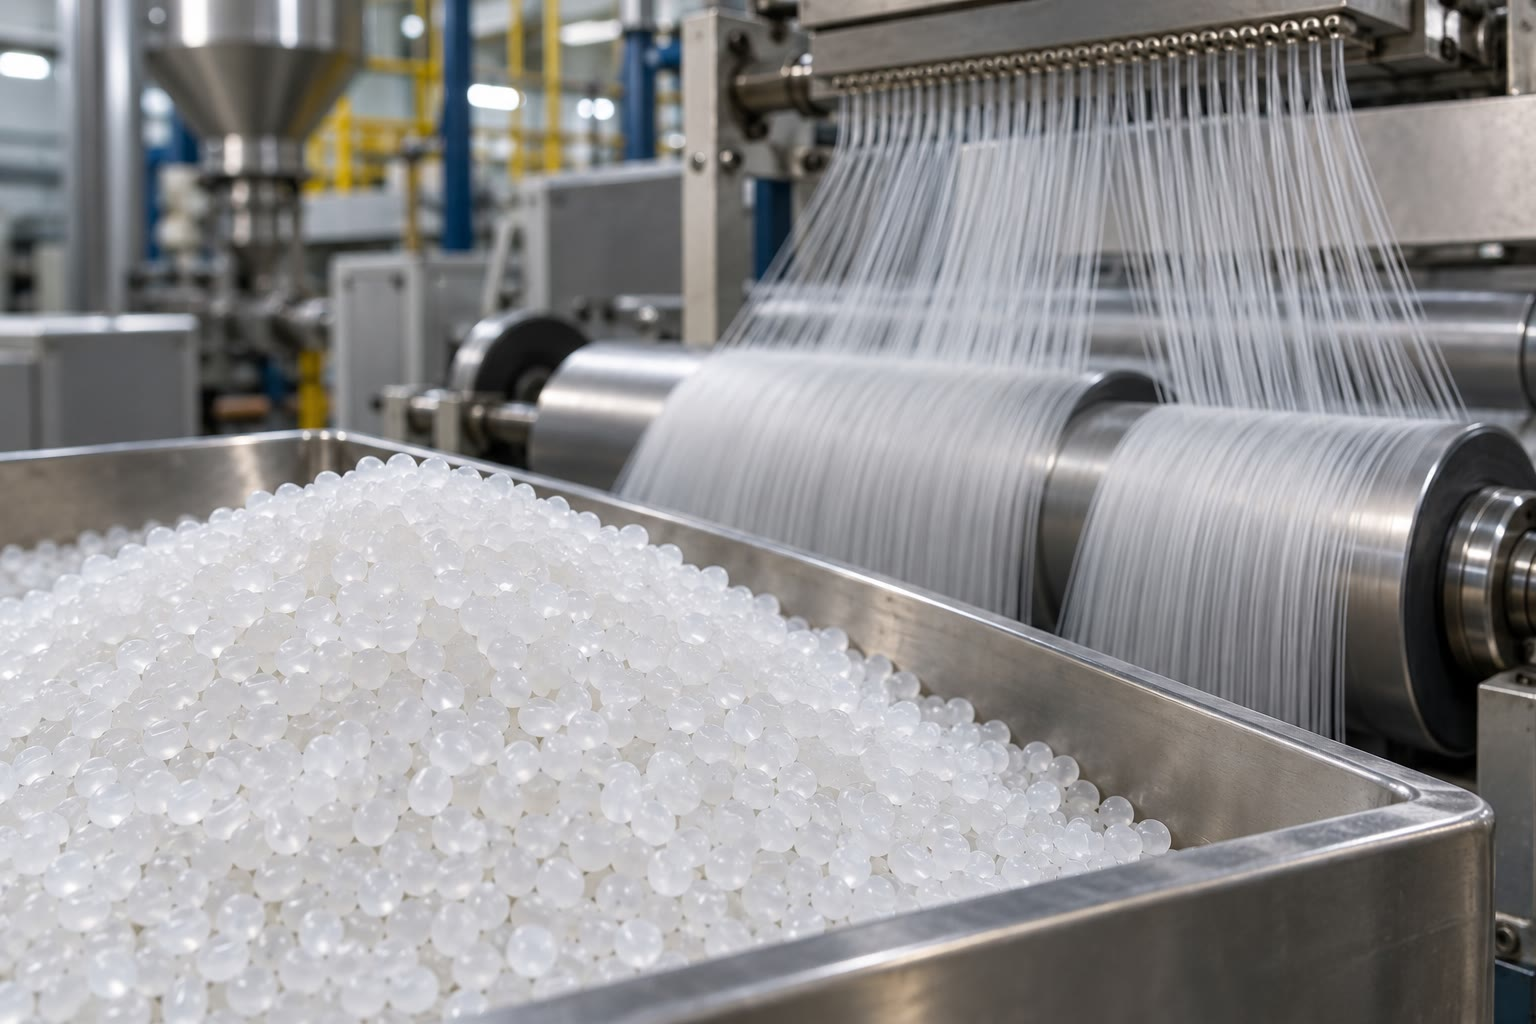
\includegraphics[width=0.58\linewidth]{images/book3/ai/b2-29-pellets.jpg}

{\small किसी संयंत्र में \omterm{def:b2:polymer-synthesis:polymer}{बहुलक} के दाने, जिस रूप में थर्मोप्लास्टिक बेचे जाते हैं, और उनके पीछे एक स्पिनरेट से
घूमते बेलनों पर खींचे जाते रेशे (चित्रण)।}
\end{omfigure}

\begin{history}[99~\% लब्धि पर्याप्त नहीं]
\begin{minipage}[t]{0.2\linewidth}
\vspace{0pt}
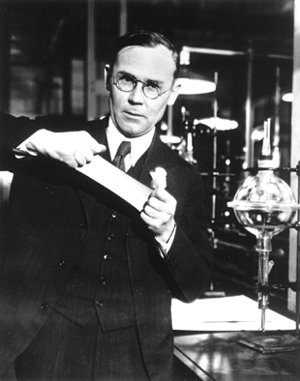
\includegraphics[width=\linewidth]{images/book3/carothers.jpg}
\end{minipage}\hfill
\begin{minipage}[t]{0.76\linewidth}
\vspace{0pt}
वॉलेस कैरोदर्स, एक युवा विश्वविद्यालय प्रशिक्षक जिन्हें मौलिक अनुसंधान के लिए एक औद्योगिक प्रयोगशाला में भर्ती किया गया था,
सुपरिचित अभिक्रियाओं से लंबे अणु बनाते गए, और उनके परिणामों ने उस समय विवादित इस विचार का दृढ़ता से
समर्थन किया कि \omterm{def:b2:polymer-synthesis:polymer}{बहुलक} साधारण अणु ही हैं, केवल बहुत लंबे। उनकी टीम ने
पहले पॉलिएस्टर बनाए, फिर, 1934 से, पॉलिऐमाइड; उनके नाम वाला समीकरण समझाता है कि केवल
अत्यधिक \omterm{def:b2:continuous-reactors:conversion}{रूपांतरणों} ने ही रेशे क्यों दिए। नायलॉन का उत्पादन 1939 में आरंभ हुआ। (छायाचित्र: अज्ञात
छायाकार, सार्वजनिक अधिकार-क्षेत्र; विकिमीडिया कॉमन्स।)
% ledger: hist:polyamides-1934, hist:nylon-production-1939
\end{minipage}
\end{history}

\begin{safety}{\ghs[5mm]{GHS01}\,\ghs[5mm]{GHS02}\,\ghs[5mm]{GHS05}\,\ghs[5mm]{GHS07}\,\ghs[5mm]{GHS08}\,\ghs[5mm]{GHS09}}
स्टाइरीन ज्वलनशील और स्वास्थ्य के लिए ख़तरनाक है। डाइबेन्ज़ॉयल परॉक्साइड शुष्क होने पर विस्फोटक ऑक्सीकारक है और उसे
नम और ठंडा रखा जाता है। हेक्सेन-1,6-डाइऐमीन और हेक्सेनडाइओइक अम्ल आँखों के लिए संक्षारक हैं।
% ledger: ghs:styrene, ghs:BPO, ghs:hexanediamine, ghs:adipic-acid
\end{safety}

\section{अभ्यास}

\begin{exercise}[$\star$]\label{exo:b2:polymer-synthesis:1}
पॉलिएथीन, पॉलिप्रोपीन, पॉली(वाइनिल क्लोराइड), पॉलिस्टाइरीन और नायलॉन-6,6 की पुनरावृत्त इकाइयाँ खींचिए।
\end{exercise}

\begin{exercise}[$\star$]\label{exo:b2:polymer-synthesis:2}
चरण-वृद्धि या शृंखला-वृद्धि: एथेन-1,2-डाइऑल और बेन्ज़ीन-1,4-डाइकार्बोक्सिलिक अम्ल से PET; पॉलिस्टाइरीन;
नायलॉन-6,6; पॉली(मेथिल मेथैक्रिलेट); 2-हाइड्रॉक्सीप्रोपेनोइक अम्ल से पॉली(लैक्टिक अम्ल)?
\end{exercise}

\begin{exercise}[$\star$]\label{exo:b2:polymer-synthesis:3}
किसी पॉलिस्टाइरीन का $\bar X_n = 1000$ है। अंत्य समूहों की उपेक्षा करते हुए $\bar M_n$ परिकलित कीजिए।
\end{exercise}

\begin{exercise}[$\star$]\label{exo:b2:polymer-synthesis:4}
समतलीय टेढ़ी-मेढ़ी रेखा के रूप में खींची गई किसी पॉलिप्रोपीन शृंखला के मेथिल समूह पाठक की ओर, फिर
दूर, फिर ओर, फिर दूर, इत्यादि हैं। इसकी \omterm{def:b2:polymer-synthesis:tacticity}{टैक्टिसिटी} का नाम बताइए। क्या यह क्रिस्टलित हो सकती है?
\end{exercise}

\begin{exercise}[$\star\star$]\label{exo:b2:polymer-synthesis:5}
कोई नमूना दो अंशों के समान द्रव्यमानों का मिश्रण है, जिनके मोलर द्रव्यमान \qty{10}{kg/mol} और
\qty{100}{kg/mol} हैं। $\bar M_n$, $\bar M_w$ और \omterm{def:b2:polymer-synthesis:averages}{परिक्षेपिता} परिकलित कीजिए।
\end{exercise}

\begin{exercise}[$\star\star$]\label{exo:b2:polymer-synthesis:6}
किसी संतुलित \omterm{def:b2:polymer-synthesis:step-chain}{चरण-वृद्धि बहुलकीकरण} के लिए $\bar X_n$ परिकलित कीजिए, $p = 0.98$ और $p = 0.995$ पर।
\end{exercise}

\begin{exercise}[$\star\star$]\label{exo:b2:polymer-synthesis:7}
किसी डाइअम्ल और किसी डाइऐमीन को डाइऐमीन के 1~\% आधिक्य (मोलों में) के साथ मिलाया जाता है। प्राप्त किया जा सकने वाला
सबसे बड़ा $\bar X_n$ क्या है?
\end{exercise}

\begin{exercise}[$\star\star$]\label{exo:b2:polymer-synthesis:8}
किसी मूलक बहुलकीकरण में आरंभक की सांद्रता दुगुनी कर दी जाती है। बहुलकीकरण की दर और
\omterm{def:b2:polymer-synthesis:chain-length}{गतिक शृंखला लंबाई} किस गुणक से बदलती हैं?
\end{exercise}

\begin{exercise}[$\star\star$]\label{exo:b2:polymer-synthesis:9}
पॉली(वाइनिल क्लोराइड) दृढ़ है; इससे बने बग़ीचे के पाइप लचीले होते हैं क्योंकि उनमें एक सुघट्यकारी होता है,
शृंखलाओं के बीच मिलाया गया एक छोटा अणु। काँच संक्रमण से समझाइए।
\end{exercise}

\begin{exercise}[$\star\star\star$]\label{exo:b2:polymer-synthesis:10}
दिखाइए कि फ़्लोरी द्रव्यमान वितरण $w_x = x(1-p)^2p^{\,x-1}$, सतत $x$ के फलन के रूप में देखने पर,
$x = -1/\ln p$ पर सबसे बड़ा है, और यह कि यह $\bar X_n$ के निकट है जब $p$ 1 के निकट हो।
\end{exercise}

\begin{exercise}[$\star\star\star$]\label{exo:b2:polymer-synthesis:11}
PET दो चरणों में बनता है: आधिक्य एथेन-1,2-डाइऑल के साथ डाइमेथिल बेन्ज़ीन-1,4-डाइकार्बोक्सिलेट
बिस(2-हाइड्रॉक्सीएथिल) बेन्ज़ीन-1,4-डाइकार्बोक्सिलेट और मेथेनॉल देता है; फिर इस डाइएस्टर को निर्वात में गर्म किया जाता है
और यह एथेन-1,2-डाइऑल मुक्त करते हुए बहुलकित होता है। दोनों चरण लिखिए और समझाइए कि दूसरा चरण
कैरोदर्स समीकरण की रससमीकरणमिति समस्या को कैसे हल करता है।
\end{exercise}

\begin{exercise}[$\star\star\star$]\label{exo:b2:polymer-synthesis:12}
\omterm{def:b2:polymer-synthesis:polymer}{एकलकों} 1 और 2 के किसी मूलक सहबहुलकीकरण में \omterm{def:b2:polymer-synthesis:copolymer}{सहबहुलक} का तात्क्षणिक संघटन
$\dfrac{\mathrm d[\mathrm M_1]}{\mathrm d[\mathrm M_2]} = \dfrac{[\mathrm M_1](r_1[\mathrm M_1]
+ [\mathrm M_2])}{[\mathrm M_2]([\mathrm M_1] + r_2[\mathrm M_2])}$ से दिया जाता है, जहाँ $r_1$ और $r_2$
अभिक्रियाशीलता अनुपात हैं (अभ्यास के आँकड़े: $r_1 = 2.0$, $r_2 = 0.5$)। समान-मोलर भरण से बने \omterm{def:b2:polymer-synthesis:copolymer}{सहबहुलक} में
इकाइयों का अनुपात परिकलित कीजिए। यदि $r_1 = r_2 = 0$ हो तो क्या होता है?
\end{exercise}

\section{समस्या: किलोग्राम के हिसाब से नायलॉन-6,6}

\begin{problem}[{सप्ताहांत समस्या --- एकलक और नायलॉन लवण, कैरोदर्स समीकरण, एक
सोचा-समझा असंतुलन, फ़्लोरी वितरण और मुक्त जल}]
\label{pb:b2:polymer-synthesis:1}
नायलॉन-6,6 हेक्सेन-1,6-डाइऐमीन और हेक्सेनडाइओइक अम्ल से बनता है। पूरी समस्या में अंत्य समूहों की उपेक्षा की गई है।
मोलर द्रव्यमान (\unit{g/mol}): C 12.011, H 1.008, N 14.007, O 15.999।
% ledger: aw:C, aw:H, aw:N, aw:O, ghs:hexanediamine, ghs:adipic-acid

\medskip
\noindent\textbf{भाग I --- \omterm{def:b2:polymer-synthesis:polymer}{एकलक} और \omterm{def:b2:polymer-synthesis:polymer}{पुनरावृत्त इकाई}।}
\begin{enumerate}
  \item दोनों \omterm{def:b2:polymer-synthesis:polymer}{एकलकों} के सूत्र लिखिए।
  \item एक ऐमाइड कड़ी बनने का समीकरण लिखिए।
  \item \omterm{def:b2:polymer-synthesis:polymer}{एकलकों} को पहले 1\,:\,1 लवण के रूप में संयोजित किया जाता है, जो विलयन से क्रिस्टलित होता है। क्यों?
  \item नायलॉन-6,6 की \omterm{def:b2:polymer-synthesis:polymer}{पुनरावृत्त इकाई}, उसका सूत्र और उसका मोलर द्रव्यमान दीजिए।
  \item शृंखला में किसी एकलक-व्युत्पन्न इकाई का माध्य मोलर द्रव्यमान $M_0$ क्या है?
  \item नाम ``6,6'' की दोनों संख्याएँ क्या गिनती हैं?
\end{enumerate}

\medskip
\noindent\textbf{भाग II --- कैरोदर्स समीकरण।}
\begin{enumerate}[resume]
  \item $\bar X_n$ और $\bar M_n$ परिकलित कीजिए, $p = 0.98$ पर।
  \item $p = 0.99$ पर वही।
  \item टिप्पणी ``99~\% लब्धि पर्याप्त नहीं'' को समझाइए।
  \item अभिक्रिया की कौन-सी प्रगति $\bar M_n = \qty{10}{kg/mol}$ देती है?
  \item व्यवहार में प्रगति को इतना ऊँचा कैसे धकेला जाता है?
  \item \omterm{def:b2:polymer-synthesis:polymer}{एकलकों} का अत्यंत शुद्ध होना क्यों आवश्यक है?
\end{enumerate}

\medskip
\noindent\textbf{भाग III --- सोचा-समझा असंतुलन।}
\begin{enumerate}[resume]
  \item डाइऐमीन 1~\% मोलर आधिक्य में प्रयुक्त होता है। $r$ परिकलित कीजिए।
  \item तब प्राप्त किए जा सकने वाले सबसे बड़े $\bar X_n$ और $\bar M_n$ परिकलित कीजिए।
  \item इस असंतुलन के साथ $\bar X_n$ परिकलित कीजिए, $p = 0.99$ पर।
  \item अभिक्रिया के अंत में कौन-से समूह शृंखलाओं को समाप्त करते हैं?
  \item कभी-कभी थोड़ा एथेनोइक अम्ल मिलाया जाता है। यह शृंखलाओं के साथ क्या करता है?
  \item कोई निर्माता जान-बूझकर शृंखला की लंबाई सीमित क्यों करेगा?
\end{enumerate}

\medskip
\noindent\textbf{भाग IV --- वितरण और द्रव्यमान संतुलन।}
\begin{enumerate}[resume]
  \item $p = 0.99$ पर किसी संतुलित मिश्रण के लिए \omterm{def:b2:polymer-synthesis:averages}{परिक्षेपिता} दीजिए।
  \item $\bar M_w$ परिकलित कीजिए, $p = 0.99$ पर।
  \item $p = 0.99$ पर अणुओं का कितना अंश, और द्रव्यमान का कितना अंश, अभी भी
        अनभिक्रियित \omterm{def:b2:polymer-synthesis:polymer}{एकलक} है?
  \item द्रव्यमान वितरण किस शृंखला लंबाई के निकट सबसे बड़ा है?
  \item नायलॉन-6,6 के प्रति किलोग्राम मुक्त जल का द्रव्यमान परिकलित कीजिए।
  \item गलित कताई को किसी परास के भीतर $\bar M_n$ क्यों चाहिए?
  \item किसी संतुलित मिश्रण के लिए $\bar M_n = \qty{20}{kg/mol}$ देने वाली अभिक्रिया की प्रगति बताइए।
\end{enumerate}
\end{problem}
